% hopforge: feature overview (Beamer, compile with xelatex)
\documentclass[aspectratio=169,11pt]{beamer}
\usetheme[progressbar=frametitle,numbering=fraction,block=fill]{metropolis}
\usepackage{fontspec}
\setsansfont{Inter}[BoldFont={Inter SemiBold}]
\setmonofont{DejaVu Sans Mono}[Scale=0.8]
\usepackage{amsmath,amssymb,bm,booktabs,tabularx,listings,tikz,qrcode,array}
\usetikzlibrary{positioning,arrows.meta,shapes.geometric,fit,calc}

% ---------- palette ----------
\definecolor{navy}{HTML}{14213D}
\definecolor{accent}{HTML}{E76F51}
\definecolor{teal}{HTML}{2A9D8F}
\definecolor{sand}{HTML}{F4F1EA}
\definecolor{grayt}{HTML}{6B7280}
\setbeamercolor{frametitle}{bg=navy,fg=white}
\setbeamercolor{progress bar}{fg=accent,bg=navy!25}
\setbeamercolor{normal text}{fg=navy!95!black,bg=white}
\setbeamercolor{alerted text}{fg=accent}
\setbeamercolor{background canvas}{bg=white}
\setbeamercolor{block title}{bg=navy!12,fg=navy}
\setbeamercolor{block body}{bg=sand}
\setbeamercolor{section in toc}{fg=navy}
\setbeamerfont{frametitle}{size=\large,series=\bfseries}
\setbeamertemplate{itemize item}{\color{accent}\scriptsize$\blacksquare$}
\setbeamertemplate{itemize subitem}{\color{teal}\tiny$\blacktriangleright$}

% ---------- colour code for physical quantities and operators ----------
\definecolor{cHam}{HTML}{1D4ED8}   % Hamiltonians
\definecolor{cHop}{HTML}{D97706}   % hoppings / couplings
\definecolor{cSpin}{HTML}{059669}  % spin operators
\definecolor{cOrb}{HTML}{7C3AED}   % orbital operators
\definecolor{cBerry}{HTML}{DC2626} % Berry curvature / connection
\definecolor{cVel}{HTML}{0891B2}   % velocities / currents
\definecolor{cGreen}{HTML}{BE185D} % Green's functions / self-energies
\definecolor{cE}{HTML}{4B5563}     % energies, chemical potential
\newcommand{\Hm}[1]{{\color{cHam}#1}}
\newcommand{\Hp}[1]{{\color{cHop}#1}}
\newcommand{\Sp}[1]{{\color{cSpin}#1}}
\newcommand{\Lo}[1]{{\color{cOrb}#1}}
\newcommand{\Bc}[1]{{\color{cBerry}#1}}
\newcommand{\Ve}[1]{{\color{cVel}#1}}
\newcommand{\Gf}[1]{{\color{cGreen}#1}}
\newcommand{\En}[1]{{\color{cE}#1}}

% ---------- code ----------
\definecolor{codebg}{HTML}{F8FAFC}
\lstdefinestyle{py}{language=Python,basicstyle=\ttfamily\footnotesize,keywordstyle=\color{cHam}\bfseries,
  commentstyle=\color{grayt}\itshape,stringstyle=\color{teal},backgroundcolor=\color{codebg},frame=leftline,
  rulecolor=\color{accent},framerule=2pt,xleftmargin=6pt,framexleftmargin=4pt,showstringspaces=false,
  columns=fullflexible,keepspaces=true,upquote=true,
  literate={²}{{$^2$}}1 {θ}{{$\theta$}}1 {λ}{{$\lambda$}}1 {Δ}{{$\Delta$}}1 {μ}{{$\mu$}}1}
\lstset{style=py}

\tikzset{box/.style={rounded corners=3pt,draw=none,fill=#1,text=white,font=\scriptsize\bfseries,align=center,minimum height=0.66cm,minimum width=1.8cm,inner sep=1.5pt},
  arr/.style={-{Stealth[length=5pt]},thick,navy!50},
  st/.style={rounded corners=2pt,fill=#1,text=white,font=\scriptsize\bfseries,minimum width=4.6cm,minimum height=0.42cm}}
\newcommand{\fig}[2][]{\includegraphics[#1]{fig/#2}}
\newcommand{\figcap}[1]{\par\vspace{1pt}{\scriptsize\color{grayt}#1}}
\newcommand{\badge}[2]{\tikz[baseline=(b.base)]\node[fill=#1,text=white,rounded corners=2pt,inner sep=2.5pt,font=\scriptsize\bfseries](b){#2};}
\newcommand{\stat}[2]{\begin{tikzpicture}\node[fill=sand,rounded corners=4pt,minimum width=2.3cm,minimum height=1.45cm,align=center]{{\Large\bfseries\color{accent}#1}\\[1pt]{\scriptsize\color{navy}#2}};\end{tikzpicture}}

\title{\textbf{hopforge}}
\subtitle{A universal tight-binding engine: models, topology, response, quantum transport,\\ strong correlations and moiré physics in one Python package}
\author{Gokaran Shukla}
\institute{King Abdullah University of Science and Technology (KAUST)\\\texttt{github.com/Gokaran-Shukla/hopforge}}
\date{Version 0.8.0 \textbullet{} November 2026}

\begin{document}

{\setbeamercolor{background canvas}{bg=navy}\setbeamercolor{normal text}{fg=white}\usebeamercolor[fg]{normal text}
\begin{frame}[plain]
\begin{tikzpicture}[remember picture,overlay]
  % decorative honeycomb
  \foreach \i in {0,...,7}{\foreach \j in {0,...,5}{
    \pgfmathsetmacro{\x}{11.2+\i*0.75+mod(\j,2)*0.375}\pgfmathsetmacro{\y}{0.6+\j*0.65}
    \node[regular polygon,regular polygon sides=6,draw=white!25,minimum size=0.82cm,line width=0.5pt] at (\x,\y){};}}
  \foreach \p in {(12.7,2.55),(13.45,3.2),(14.2,2.55),(13.08,1.9)}{\fill[accent] \p circle (3pt);}
  \node[anchor=north west,text width=11cm,text=white,align=left] at ([xshift=1.1cm,yshift=-1.4cm]current page.north west){
    {\fontsize{44}{48}\selectfont\bfseries hop\textcolor{accent}{forge}}\\[6pt]
    {\large A universal tight-binding engine}\\[3pt]
    {\normalsize\color{white!75}models \textbullet{} topology \textbullet{} linear response \textbullet{} quantum transport\\
     strong correlations \textbullet{} quantum phases \textbullet{} moiré \& orbitronics}\\[22pt]
    {\normalsize\bfseries Gokaran Shukla}\\[2pt]
    {\small\color{white!75}KAUST \textbullet{} v0.8.0 \textbullet{} November 2026}\\[2pt]{\small\color{accent}github.com/Gokaran-Shukla/hopforge}};
\end{tikzpicture}
\end{frame}
}

\begin{frame}{hopforge at a glance}
\centering
\stat{36}{benchmarked models}\hfill\stat{77/77}{published benchmarks}\hfill\stat{140}{automated tests}\hfill\stat{24}{executed tutorials}\hfill\stat{480}{quiz questions}
\vspace{10pt}
\begin{columns}[T]
\begin{column}{0.5\textwidth}
\begin{itemize}\small
\item \textbf{Any} tight-binding model: 0D--3D, spinful, matrix hoppings, Slater-Koster $s/p/d$, $k\!\cdot\!p$ discretisation, Wannier90
\item \textbf{One model, every tool}: bands, topology, Kubo, Boltzmann, Landauer, finite-bias NEGF, KPM, surfaces, ED, DMRG, Floquet
\item \textbf{Parallel} on a full node (\texttt{n\_jobs=40}) or on a GPU (\texttt{backend.use("cupy")})
\end{itemize}
\end{column}
\begin{column}{0.5\textwidth}
\begin{itemize}\small
\item \textbf{Validated}: every method checked against an analytic or published number
\item \textbf{Teachable}: tutorial + 20-question quiz per topic, four step-by-step ``build your own Hamiltonian'' notebooks
\item \textbf{Open}: MIT licence, CI on Linux/macOS, Python 3.10--3.13
\end{itemize}
\end{column}
\end{columns}
\end{frame}

\begin{frame}{Outline}
\vspace{6pt}
\begin{tabular}{@{}r@{\hspace{8pt}}p{5.6cm}r@{\hspace{8pt}}p{5.6cm}@{}}
{\color{accent}\bfseries 01} & Building Hamiltonians & {\color{accent}\bfseries 07} & Strong correlations and quantum phases\\[4pt]
{\color{accent}\bfseries 02} & Topology & {\color{accent}\bfseries 08} & DMRG, finite-bias NEGF, GPU, community\\[4pt]
{\color{accent}\bfseries 03} & Linear response & {\color{accent}\bfseries 09} & Validation\\[4pt]
{\color{accent}\bfseries 04} & Quantum transport and large-scale methods & {\color{accent}\bfseries 10} & Performance\\[4pt]
{\color{accent}\bfseries 05} & Orbitronics, torques and moiré bilayers & {\color{accent}\bfseries 11} & Learning: tutorials and quizzes\\[4pt]
{\color{accent}\bfseries 06} & Allan MacDonald's models & {\color{accent}\bfseries 12} & Status and outlook\\[4pt]
\end{tabular}
\end{frame}

\begin{frame}{Colour convention used in the equations}
\begin{columns}[c]
\begin{column}{0.44\textwidth}
\small\renewcommand{\arraystretch}{1.4}
\begin{tabular}{@{}>{\centering\arraybackslash}p{1.5cm}l@{}}
\toprule
$\Hm{H}$, $\Hm{H(\mathbf k)}$ & Hamiltonians\\
$\Hp{t},\Hp{\lambda},\Hp{U},\Hp{J}$ & hoppings and couplings\\
$\Sp{\sigma},\Sp{\mathbf S}$ & spin operators\\
$\Lo{\mathbf L}$ & orbital angular momentum\\
$\Bc{\Omega},\Bc{\mathcal A}$ & Berry curvature, connection\\
$\Ve{v},\Ve{J}$ & velocities and currents\\
$\Gf{G},\Gf{\Sigma}$ & Green's functions, $\Sigma$\\
$\En{E},\En{\mu},\En{\Gamma}$ & energies, broadening\\
\bottomrule
\end{tabular}
\end{column}
\begin{column}{0.52\textwidth}
\begin{block}{Conventions in the code}
\small
\begin{itemize}
\item atomic gauge $\Hm{H_{ij}(\mathbf k)}=\sum_{\mathbf R}\Hp{t_{ij}(\mathbf R)}\,e^{i\mathbf k\cdot(\mathbf R+\mathbf r_j-\mathbf r_i)}$ (periodic gauge optional)
\item spin basis orbital-major: index $=2\,\text{orb}+s$
\item $\hbar=e=k_B=1$; Hall responses in $e^2/h$ (2D) or S/cm (3D)
\item Wannier90 sign of $\sigma_{xy}=-C\,e^2/h$
\end{itemize}
\end{block}
\end{column}
\end{columns}
\end{frame}

\begin{frame}{Architecture: one model object, many solvers}
\centering
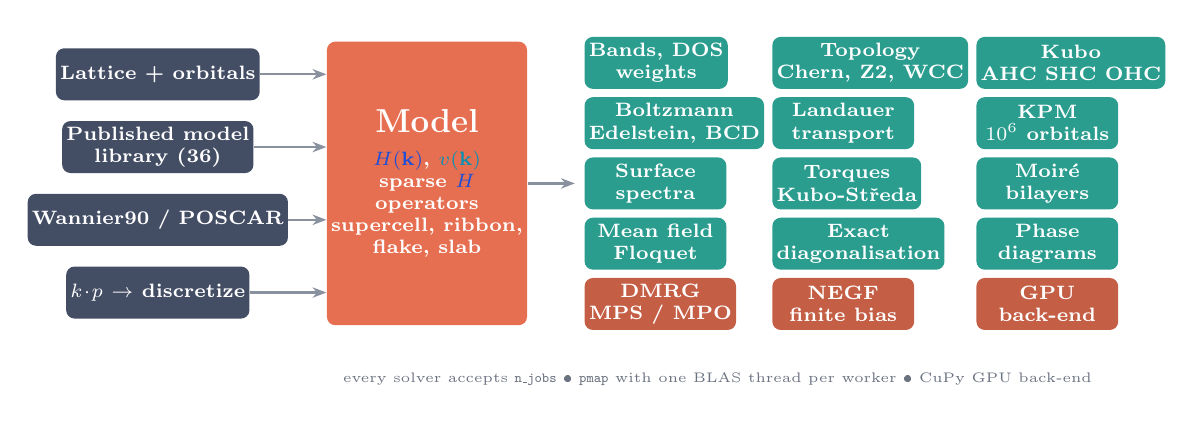
\begin{tikzpicture}
\node[box=navy!80](inp1){Lattice + orbitals};
\node[box=navy!80,below=0.25 of inp1](inp2){Published model\\library (36)};
\node[box=navy!80,below=0.25 of inp2](inp3){Wannier90 / POSCAR};
\node[box=navy!80,below=0.25 of inp3](inp4){$k\!\cdot\!p$ $\to$ discretize};
\node[box=accent,minimum height=3.6cm,minimum width=2.4cm,right=0.7 of $(inp2.east)!0.5!(inp3.east)$](M){\large Model\\[4pt]\scriptsize $\Hm{H(\mathbf k)}$, $\Ve{v(\mathbf k)}$\\sparse $\Hm{H}$\\operators\\supercell, ribbon,\\flake, slab};
\foreach \n in {inp1,inp2,inp3,inp4}{\draw[arr](\n.east)--(M.west|-\n.east);}
\matrix[right=0.6 of M,row sep=3pt,column sep=3pt,ampersand replacement=\&](S){
\node[box=teal]{Bands, DOS\\weights};\&\node[box=teal]{Topology\\Chern, Z2, WCC};\&\node[box=teal]{Kubo\\AHC SHC OHC};\\
\node[box=teal]{Boltzmann\\Edelstein, BCD};\&\node[box=teal]{Landauer\\transport};\&\node[box=teal]{KPM\\$10^6$ orbitals};\\
\node[box=teal]{Surface\\spectra};\&\node[box=teal]{Torques\\Kubo-Středa};\&\node[box=teal]{Moiré\\bilayers};\\
\node[box=teal]{Mean field\\Floquet};\&\node[box=teal]{Exact\\diagonalisation};\&\node[box=teal]{Phase\\diagrams};\\
\node[box=accent!85!black]{DMRG\\MPS / MPO};\&\node[box=accent!85!black]{NEGF\\finite bias};\&\node[box=accent!85!black]{GPU\\back-end};\\};
\draw[arr](M.east)--(S.west);
\node[below=0.3 of S,font=\tiny,text=grayt,xshift=-2cm]{every solver accepts \texttt{n\_jobs} \textbullet{} \texttt{pmap} with one BLAS thread per worker \textbullet{} CuPy GPU back-end};
\end{tikzpicture}
\end{frame}

% =====================================================================
\section{Building Hamiltonians}

\begin{frame}[fragile]{A model in five lines, with neighbour shells drawn}
\begin{columns}[c]
\begin{column}{0.52\textwidth}
\begin{lstlisting}
import hopforge as hf, numpy as np
lat = hf.Lattice([[1, 0], [0, 1]],
      [("Cu", [0, 0]), ("Ox", [.5, 0]),
       ("Oy", [0, .5])])
m = hf.Model(lat, spinful=True)
m.add_neighbors(-1.0, shell=1)
m.add_slater_koster({"pps": 1, "ppp": -.3}, 2)
m.add_rashba(0.1); m.add_exchange(0.6, (0,0,1))
hf.plot_lattice(m, shells=3)
\end{lstlisting}
\vspace{2pt}
\footnotesize
\begin{itemize}
\item h.c.\ automatic; matrix hoppings; Slater-Koster $s,p,d$ along any bond
\item SOC $\Hp{\lambda}\,\Lo{\mathbf L}\cdot\Sp{\mathbf S}$, Rashba, exchange, Peierls phases
\end{itemize}
\end{column}
\begin{column}{0.46\textwidth}
\centering\fig[width=\linewidth]{shells.png}
\figcap{1st/2nd/3rd shells with distances and coordination numbers}
\end{column}
\end{columns}
\end{frame}

\begin{frame}{The model library: 36 published Hamiltonians}
\scriptsize
\renewcommand{\arraystretch}{1.12}
\begin{tabularx}{\textwidth}{@{}>{\bfseries\color{accent}}l X@{}}
\toprule
1D & chain, SSH, Rice-Mele, Kitaev chain, Creutz ladder\\
2D lattices & square, triangular, honeycomb, kagome, Lieb, checkerboard, dice, bilayer graphene, pyrochlore (3D)\\
Topological & Haldane, Kane-Mele, Qi-Wu-Zhang, BHZ, Hofstadter, Wilson-Dirac TI, Fu-Kane-Mele diamond, minimal Weyl\\
Spintronics & Rashba square, $d$-wave altermagnet, $p$-orbital square (orbital Hall), exchange-split models\\
3D crystals & cubic, bcc, fcc, diamond, Vogl $sp^3s^*$ silicon (Slater-Koster engine)\\
Bernevig group & BBH quadrupole insulator, chiral $p+ip$ superconductor, type-II Weyl, flat Chern band, BHZ\\
Vishwanath / moiré & Bistritzer-MacDonald and chiral TBG, real-space twisted bilayers (Moon-Koshino)\\
MacDonald group & TMD moiré Hubbard and topological MoTe$_2$ bands, ABC $N$-layer graphene, graphene QAH, Rashba 2DEG spin Hall\\
Sachdev / correlated & SYK, transverse-field Ising, Hubbard, Kanamori, Bose-Hubbard, Kitaev honeycomb\\
Builders & \texttt{bdg()}, \texttt{make\_spinful()}, \texttt{discretize()}, \texttt{bilayer()}, \texttt{register\_model} for community models\\
\bottomrule
\end{tabularx}
\end{frame}

\begin{frame}{Spectra with operator weights}
\centering
\begin{minipage}[t]{0.32\textwidth}\centering\fig[height=3.8cm]{altermagnet.png}\figcap{$d$-wave altermagnet, colour $\langle\Sp{S_z}\rangle$}\end{minipage}\hfill
\begin{minipage}[t]{0.32\textwidth}\centering\fig[height=3.8cm]{porbital.png}\figcap{$p$-orbital square, colour $\langle\Lo{L_z}\rangle$ texture}\end{minipage}\hfill
\begin{minipage}[t]{0.32\textwidth}\centering\fig[height=3.8cm]{hofstadter.png}\figcap{Hofstadter butterfly from Peierls phases}\end{minipage}

\vspace{10pt}
\footnotesize Bands, DOS/PDOS, Fermi level and gaps; weights of any operator ($\Sp{\sigma}$, $\Lo{\mathbf L}$, layer, sublattice, projector).
\end{frame}

\begin{frame}{From DFT and from $k\cdot p$}
\begin{columns}[c]
\begin{column}{0.5\textwidth}
\begin{block}{Wannier90 interface}
\small \texttt{read\_wannier90(hr.dat, lattice=POSCAR, positions=centres.xyz, spinful=True)}\\[2pt]
spin ordering interleaved/block; \texttt{tb.dat}, \texttt{.win}; \texttt{hr.dat} export
\end{block}
\begin{block}{Continuum to lattice}
\small
\texttt{hf.discretize("C*(k\_x**2+k\_y**2) + A*(k\_x*sigma\_x + k\_y*sigma\_y) + M*sigma\_z")}\\[3pt]
$\Hm{H(\mathbf k)}$ with non-commuting $\Sp{\sigma},\tau$ symbols; Kronecker products automatic
\end{block}
\end{column}
\begin{column}{0.46\textwidth}
\centering\fig[width=\linewidth]{discretize.png}
\figcap{discretised bands converge to the continuum as $a\to0$}
\end{column}
\end{columns}
\end{frame}

% =====================================================================
\section{Topology}

\begin{frame}{Topological invariants}
\begin{columns}[T]
\begin{column}{0.36\textwidth}
\small
\textbf{Chern number} (Fukui-Hatsugai-Suzuki)
\[C=\frac{1}{2\pi}\int_{\rm BZ}\Bc{\Omega_{xy}(\mathbf k)}\,d^2k\]
\textbf{Wilson loop} / hybrid Wannier centres
\[W=\prod_{j}P(\mathbf k_j),\quad \bar x=\tfrac{1}{2\pi}\arg\lambda_W\]
\begin{itemize}\scriptsize
\item Berry/Zak phase, polarisation, pumping
\item 2D and 3D Z2, Fu-Kane parity
\item winding numbers, nested Wilson loops
\end{itemize}
\end{column}
\begin{column}{0.31\textwidth}\centering\fig[width=\linewidth]{haldane_pd.png}\figcap{Haldane phase diagram (Chern number)}\end{column}
\begin{column}{0.31\textwidth}\centering\fig[width=\linewidth]{wcc.png}\figcap{Kramers partner switching, Z2 = 1}\end{column}
\end{columns}
\end{frame}

\begin{frame}{Bulk-boundary correspondence: edges, surfaces, corners}
\centering
\begin{minipage}[t]{0.24\textwidth}\centering\fig[width=0.95\linewidth]{haldane_ribbon.png}\figcap{chiral edge states (Haldane ribbon)}\end{minipage}\hfill
\begin{minipage}[t]{0.24\textwidth}\centering\fig[width=0.95\linewidth]{km_spectral.png}\figcap{surface Green's function, Kane-Mele}\end{minipage}\hfill
\begin{minipage}[t]{0.24\textwidth}\centering\fig[width=0.95\linewidth]{fermi_arc.png}\figcap{Fermi arc of a Weyl semimetal}\end{minipage}\hfill
\begin{minipage}[t]{0.24\textwidth}\centering\fig[width=0.95\linewidth]{bbh.png}\figcap{BBH corner charges $\pm e/2$}\end{minipage}

\vspace{10pt}
\footnotesize WannierTools-style surface spectral functions via Sancho-Rubio decimation $\Gf{G_s}(\En{E},\mathbf k_\parallel)$, spin-resolved, batched over energies; nested Wilson loop gives $p_y^{\nu_x}=1/2$ for the quadrupole insulator.
\end{frame}

% =====================================================================
\section{Linear response}

\begin{frame}{Kubo: anomalous, spin and orbital Hall conductivities}
\begin{columns}[c]
\begin{column}{0.4\textwidth}
\small
\[\sigma^{\gamma}_{xy}=-\frac{e}{\hbar}\sum_{n\mathbf k}f_{n\mathbf k}\,\Bc{\Omega^{\gamma}_{n}(\mathbf k)}\]
\[\Bc{\Omega^{\gamma}_{n}}=2\hbar^2\sum_{m\neq n}\mathrm{Im}\frac{\langle n|\Ve{J^{\gamma}_x}|m\rangle\langle m|\Ve{v_y}|n\rangle}{(\En{E_n}-\En{E_m})^2}\]
with $\Ve{J^{\gamma}_x}=\tfrac12\{\Ve{v_x},O^\gamma\}$, $O^\gamma\in\{1,\Sp{S_z},\Lo{L_z}\}$
\begin{itemize}\scriptsize
\item Haldane: $\sigma_{xy}=-1\,e^2/h$ plateau
\item orbital Hall without SOC (Go et al.\ PRL 2018)
\end{itemize}
\end{column}
\begin{column}{0.29\textwidth}\centering\fig[width=\linewidth]{haldane_ahc.png}\figcap{quantised AHC in the gap}\end{column}
\begin{column}{0.29\textwidth}\centering\fig[width=\linewidth]{ohc_shc.png}\figcap{OHC $\gg$ SHC; OHC needs no SOC}\end{column}
\end{columns}
\end{frame}

\begin{frame}{Boltzmann, Edelstein and nonlinear Hall}
\centering
\begin{minipage}[t]{0.32\textwidth}\centering\fig[width=0.9\linewidth]{powerfactor.png}\figcap{thermoelectric power factor $S^2\sigma$}\end{minipage}\hfill
\begin{minipage}[t]{0.32\textwidth}\centering\fig[width=0.9\linewidth]{orbital_edelstein.png}\figcap{orbital Rashba-Edelstein: $E_x\to\langle\Lo{L_y}\rangle$}\end{minipage}\hfill
\begin{minipage}[t]{0.32\textwidth}\centering\fig[width=0.9\linewidth]{bcd.png}\figcap{Berry curvature dipole $D_a=\sum\int f\,\partial_a\Bc{\Omega_z}$}\end{minipage}

\vspace{10pt}
\footnotesize
$\sigma_{ij}=e^2\tau\sum\int \Ve{v_i}\Ve{v_j}(-\partial_E f)$, Seebeck, $\kappa$, Lorenz number \textbullet{}
Edelstein $\delta\langle O\rangle=\chi\,E$ extrinsic ($\propto\tau$) and intrinsic \textbullet{} Drude weight
\end{frame}

\begin{frame}{Orbital magnetism and optics}
\begin{columns}[c]
\begin{column}{0.32\textwidth}\centering\fig[width=\linewidth]{orb_moment.png}\figcap{valley orbital moment of gapped graphene}\end{column}
\begin{column}{0.32\textwidth}\centering\fig[width=\linewidth]{optical.png}\figcap{universal optical conductivity $\sigma_0=e^2/4\hbar$}\end{column}
\begin{column}{0.32\textwidth}
\small
\[\Lo{m_n}=-\tfrac{ie}{2\hbar}\langle\partial_{\mathbf k}u_n|\times[\Hm{H}-\En{E_n}]|\partial_{\mathbf k}u_n\rangle\]
\begin{itemize}\scriptsize
\item modern orbital magnetisation $M(\En\mu)$; Středa slope $C/2\pi$ in the gap
\item Kubo-Greenwood $\sigma_{ab}(\omega)$, Hall limit $\omega\to0$
\end{itemize}
\end{column}
\end{columns}
\end{frame}

% =====================================================================
\section{Quantum transport and large-scale methods}

\begin{frame}[fragile]{Kwant-style scattering: shapes, leads, parameters}
\begin{columns}[c]
\begin{column}{0.53\textwidth}
\begin{lstlisting}
from hopforge import transport as tr
s = tr.System(hf.models.square(),
      lambda r: 0 <= r[0] < 60 and 0 <= r[1] < 30,
      onsite=lambda r, n, V: V*(abs(r[0]-30) < 4),
      peierls=tr.landau_gauge)
s.attach_lead((-1, 0)); s.attach_lead((1, 0))
G = s.conductance(E, params=dict(V=.5, B=.02),
                  n_jobs=40)
S = s.smatrix(-1.0); S.shot_noise(); S.current(0)
\end{lstlisting}
\small
\[T=\mathrm{Tr}\big[\Gamma_L\,\Gf{G^r}\,\Gamma_R\,\Gf{G^a}\big],\quad \Gamma=i(\Gf{\Sigma}-\Gf{\Sigma}^\dagger)\]
\end{column}
\begin{column}{0.45\textwidth}\centering\fig[width=\linewidth]{hallbar.png}\figcap{six-terminal Hall bar built from a shape function}
\scriptsize
\begin{itemize}
\item exact lead modes (generalised eigenproblem), Sancho-Rubio $\Gf{\Sigma}$
\item conservation laws (spin, e/h), arbitrary $B(x,y)$
\item LDOS, wavefunctions, bond currents, spectra
\end{itemize}
\end{column}
\end{columns}
\end{frame}

\begin{frame}{Landauer-Büttiker results}
\centering
\begin{minipage}[t]{0.32\textwidth}\centering\fig[width=0.9\linewidth]{qpc_steps.png}\figcap{conductance quantisation: $T$ = number of open channels}\end{minipage}\hfill
\begin{minipage}[t]{0.32\textwidth}\centering\fig[width=0.9\linewidth]{qh_plateaus.png}\figcap{quantum Hall: $R_{xy}=h/\nu e^2$, $R_{xx}=0$}\end{minipage}\hfill
\begin{minipage}[t]{0.32\textwidth}\centering\fig[width=0.9\linewidth]{edge_current.png}\figcap{bond currents follow one edge}\end{minipage}
\end{frame}

\begin{frame}{Superconductors, disorder and noise}
\centering
\begin{minipage}[t]{0.32\textwidth}\centering\fig[width=0.9\linewidth]{btk.png}\figcap{BTK Andreev doubling ($2N$) to tunnelling}\end{minipage}\hfill
\begin{minipage}[t]{0.32\textwidth}\centering\fig[width=0.9\linewidth]{tau_bimodal.png}\figcap{bimodal transmission eigenvalues, Fano $\approx1/3$}\end{minipage}\hfill
\begin{minipage}[t]{0.32\textwidth}\centering\fig[width=0.9\linewidth]{localisation.png}\figcap{Anderson localisation $\langle\ln T\rangle\propto -L/\xi$}\end{minipage}

\vspace{10pt}
\footnotesize Majorana zero-bias peak $2e^2/h$ \textbullet{} multi-terminal conductance matrices \textbullet{} four-terminal resistances \textbullet{} disorder averages in parallel
\end{frame}

\begin{frame}{Kernel polynomial method: millions of orbitals}
\begin{columns}[c]
\begin{column}{0.32\textwidth}\centering\fig[width=\linewidth]{kpm_dos.png}\figcap{graphene DOS, $9\times10^4$ sites}\end{column}
\begin{column}{0.32\textwidth}\centering\fig[width=\linewidth]{kubo_bastin.png}\figcap{disordered Chern insulator, Kubo-Bastin}\end{column}
\begin{column}{0.32\textwidth}\small
\[\rho(\En E)\approx\frac{\sum_n (2-\delta_{n0})\,g_n\mu_n T_n(\En E)}{\pi\sqrt{1-\En E^2}}\]
\[\mu_n=\tfrac1N\mathrm{Tr}\,T_n(\tilde{\Hm H})\]
\begin{itemize}\scriptsize
\item DOS, LDOS, projected DOS; Jackson/Lorentz kernels
\item Kubo-Bastin $\sigma_{xy}$ (García et al.\ 2015) with symmetry projection of stochastic noise
\item moments parallel over random vectors
\end{itemize}
\end{column}
\end{columns}
\end{frame}

% =====================================================================
\section{Orbitronics, torques and moiré bilayers}

\begin{frame}{Spin-orbit, orbital and self-torques}
\begin{columns}[c]
\begin{column}{0.38\textwidth}
\footnotesize
Kubo-Středa response of $O$ to $E_x$ (+ Fermi sea):
\[\chi^{\rm FS}=\tfrac{1}{2\pi}\mathrm{Tr}\big[O\,\Gf{G^r}\Ve{v_x}\Gf{G^a}\big]\propto\tfrac{1}{\En\Gamma}\]
Torque on $\hat m$:
\[\mathbf T=\Hp{J_{\rm ex}}\,\hat m\times\delta\langle\Sp{\mathbf S}\rangle\]
field-like $\hat m\times\hat y$, damping-like $\hat m\times(\hat y\times\hat m)$
\end{column}
\begin{column}{0.3\textwidth}\centering\fig[width=\linewidth]{ohc_light.png}\figcap{light metal: large OHC, zero SHC}\end{column}
\begin{column}{0.3\textwidth}\centering\fig[width=\linewidth]{torque_mu.png}\figcap{torque on the FM of a FM/light-metal bilayer}\end{column}
\end{columns}
\vspace{2pt}
{\scriptsize\color{grayt}Self-torque vanishes in a centrosymmetric FM (checked) and appears once interfaces break inversion, following Go \& Lee and Kurebayashi et al.}
\end{frame}

\begin{frame}{Stacked and twisted bilayers in real space}
\begin{columns}[c]
\begin{column}{0.32\textwidth}\centering\fig[width=\linewidth]{bilayer_weight.png}\figcap{FM/heavy-metal $p$-orbital bilayer, weight on the FM layer}\end{column}
\begin{column}{0.32\textwidth}\centering\fig[width=\linewidth]{moire_hall.png}\figcap{$13.17^\circ$ twisted magnetic graphene bilayer: AHC and SHC}\end{column}
\begin{column}{0.33\textwidth}\scriptsize
\begin{itemize}
\item \texttt{bilayer(bottom, top, d, interlayer)} with Slater-Koster or Moon-Koshino couplings
\item \texttt{rotate\_model} rotates the lattice, orbital $D^{l}$ blocks and the spin frame
\item commensurate angles $(m,r)$ (Lopes dos Santos)
\item layer-resolved $P\,\Sp{S}\,P$, $P\,\Lo{L}\,P$ responses and torques
\end{itemize}
\end{column}
\end{columns}
\end{frame}

\begin{frame}{Continuum moiré: magic-angle twisted bilayer graphene}
\begin{columns}[c]
\begin{column}{0.36\textwidth}
\small Bistritzer-MacDonald:
\[\Hm{H}=\begin{pmatrix}\Hm{h_{\theta/2}(\mathbf k)} & \Hp{T(\mathbf r)}\\ \Hp{T^\dagger(\mathbf r)} & \Hm{h_{-\theta/2}(\mathbf k)}\end{pmatrix}\]
$\Hp{T}=\sum_j \Hp{T_j}e^{-i\mathbf q_j\cdot\mathbf r}$, $\alpha=\Hp{w_1}/v k_\theta$\\[4pt]
\begin{itemize}\scriptsize
\item chiral limit $w_0=0$: first magic $\alpha=0.586$ (Tarnopolsky et al.)
\item real-space TBG agrees with continuum within 5\%
\end{itemize}
\end{column}
\begin{column}{0.31\textwidth}\centering\fig[width=\linewidth]{bm_velocity.png}\figcap{Dirac velocity $v^*/v$ vs $\alpha$}\end{column}
\begin{column}{0.31\textwidth}\centering\fig[width=\linewidth]{magic_flat.png}\figcap{flat bands at the magic angle}\end{column}
\end{columns}
\end{frame}

% =====================================================================
\section{Allan MacDonald's models}

\begin{frame}{MacDonald group I: TMD moiré bilayers (\texttt{hf.macdonald})}
\begin{columns}[T]
\begin{column}{0.5\textwidth}
\centering\fig[width=0.9\linewidth]{md_hetero.png}
\figcap{WSe$_2$/MoSe$_2$, 2°: top band 10.85 meV (paper $\approx$11)}
\vspace{2pt}
\fig[width=0.82\linewidth]{md_mote2.png}
\figcap{twisted MoTe$_2$: $C$ and gaps vs $\theta$ ($\theta_1^*=1.74^\circ$)}
\end{column}
\begin{column}{0.48\textwidth}
\scriptsize
\scriptsize
\textbf{Heterobilayer} (Wu, Lovorn, Tutuc \& MacDonald, PRL 2018)
\[\Hm{H}=-\tfrac{\hbar^2k^2}{2m^*}+\textstyle\sum_j \Hp{V(\mathbf b_j)}e^{i\mathbf b_j\cdot\mathbf r}\]
\vspace{-10pt}
\begin{itemize}\scriptsize
\item fit $\to$ triangular Hubbard $\Hp{t_1},\Hp{t_2},\Hp{t_3}$, harmonic $\Hp{U_0}$; \texttt{to\_model()}
\end{itemize}
\vspace{2pt}
\textbf{Homobilayer} (Wu et al., PRL 2019)
\[\Hm{H_\uparrow}=\begin{pmatrix}-\tfrac{\hbar^2(\mathbf k-\kappa_+)^2}{2m^*}+\Delta_b & \Hp{\Delta_T}\\ \Hp{\Delta_T^\dagger} & -\tfrac{\hbar^2(\mathbf k-\kappa_-)^2}{2m^*}+\Delta_t\end{pmatrix}\]
\vspace{-10pt}
\begin{itemize}\scriptsize
\item Kubo Chern numbers in the plane-wave basis
\item $C=(-1,+1)$ at 1.2°, $(-1,-1,+2)$ at 2°: QSH moiré bands
\end{itemize}
\end{column}
\end{columns}
\end{frame}

\begin{frame}{MacDonald group II: graphene multilayers, spin Hall, QAH}
\centering
\begin{minipage}[t]{0.4\textwidth}\centering\fig[width=\linewidth]{md_abc.png}\figcap{ABC graphene: $E\propto(\Ve{v}k)^N/\Hp{t_\perp}^{N-1}$ (Min \& MacDonald 2008); valley Chern $\pm N/2$}\end{minipage}\hfill
\begin{minipage}[t]{0.28\textwidth}\centering\fig[width=\linewidth]{md_sinova.png}\figcap{universal spin Hall $e/8\pi$ (Sinova et al.\ 2004): 0.995}\end{minipage}\hfill
\begin{minipage}[t]{0.28\textwidth}\centering\fig[width=\linewidth]{md_qah.png}\figcap{graphene + Rashba + exchange: QAH with $C=2$ (Tse, Qiao, Yao, MacDonald \& Niu 2011)}\end{minipage}

\vspace{8pt}
\footnotesize No public MacDonald-group tight-binding package exists; hopforge implements the published Hamiltonians and checks 10 of their results in CI. Tutorial 21 walks through all of them.
\end{frame}

% =====================================================================
\section{Strong correlations and quantum phases}

\begin{frame}{Mean-field and driven systems}
\begin{columns}[c]
\begin{column}{0.32\textwidth}\centering\fig[width=\linewidth]{neel.png}\figcap{honeycomb Néel transition $U_c\approx2.23t$}\end{column}
\begin{column}{0.32\textwidth}\centering\fig[width=\linewidth]{floquet.png}\figcap{Floquet bands of driven graphene}\end{column}
\begin{column}{0.33\textwidth}\small
\[\Hm{H_{\rm MF}}=\Hm{H_0}+\Hp{U}\big(\mathrm{Tr}\rho-\rho\big)\]
noncollinear Hartree-Fock, mixing, phase diagrams\\[4pt]
\[\Hm{H_{\rm eff}}=\Hm{H_0}+\sum_{m>0}\frac{[\Hm{H_m},\Hm{H_{-m}}]}{m\omega}\]
exact Sambe space or van Vleck; light-induced Chern insulator
\end{column}
\end{columns}
\end{frame}

\begin{frame}{Exact diagonalisation}
\begin{columns}[c]
\begin{column}{0.38\textwidth}
\small
\vspace{-6pt}\begin{align*}\Hm{H}=&-\Hp{t}\textstyle\sum c^\dagger_{i\sigma}c_{j\sigma}\\&+\Hp{U}\textstyle\sum n_{i\uparrow}n_{i\downarrow}+\Hp{V}\sum n_in_j\end{align*}
\begin{itemize}\scriptsize
\item Hubbard, extended, Kanamori ($\Hp{U},\Hp{U'},\Hp{J}$, spin flip, pair hopping)
\item spinless fermions on any lattice (FCI)
\item XXZ / $J_1$-$J_2$, Pauli strings (TFIM, Kitaev)
\item SYK $q=4$, level statistics
\item correlations, gaps, $S(\mathbf q)$, Lanczos $\Gf{G(\omega)}$
\end{itemize}
\end{column}
\begin{column}{0.3\textwidth}\centering\fig[width=\linewidth]{spectral.png}\figcap{Hubbard bands of a $2\times4$ cluster, $U=4$}\end{column}
\begin{column}{0.3\textwidth}\centering\fig[width=\linewidth]{fci.png}\figcap{$\nu=1/3$ FCI: threefold ground state}\end{column}
\end{columns}
\end{frame}

\begin{frame}{Quantum phase diagrams under doping and across criticality}
\centering
\begin{minipage}[t]{0.3\textwidth}\centering\fig[width=\linewidth]{hubbard_pd.png}\figcap{Hubbard PM/FM/AFM vs $U$ and doping}\end{minipage}\hfill
\begin{minipage}[t]{0.36\textwidth}\centering\fig[width=\linewidth]{critical.png}\figcap{TFIM: magnetisation, Binder, fidelity, entanglement}\end{minipage}\hfill
\begin{minipage}[t]{0.3\textwidth}\centering\fig[width=\linewidth]{mott.png}\figcap{Bose-Hubbard Mott lobes}\end{minipage}

\vspace{10pt}
\footnotesize Binder crossing $h_c\approx0.96$ (exact 1) \textbullet{} Calabrese-Cardy central charge $c=0.502$ \textbullet{} lobe tip $3+2\sqrt2$ \textbullet{} Stoner $\Hp{U}\rho(\En{E_F})>1$
\end{frame}

\begin{frame}{Research models: Bernevig, Vishwanath, Sachdev}
\scriptsize
\renewcommand{\arraystretch}{1.3}
\begin{tabularx}{\textwidth}{@{}l X l@{}}
\toprule
\textbf{Model} & \textbf{What hopforge reproduces} & \textbf{Reference}\\
\midrule
BHZ & Z2 phases vs $M/B$ & Science 314, 1757 (2006)\\
BBH quadrupole & nested Wilson loop $p=1/2$, corner charges $\pm e/2$ & Science 357, 61 (2017)\\
Fractional Chern insulator & threefold-degenerate $\nu=1/3$ ground state & PRX 1, 021014 (2011)\\
Flat Chern band & flatness ratio $\approx27$ & PRL 106, 236804 (2011)\\
Type-II Weyl / $p+ip$ & tilted cones; $C=\pm1$ with chiral Majoranas & Nature 527, 495; PRB 61, 10267\\
Chiral TBG & magic $\alpha=0.586$, flat bands & PRL 122, 106405 (2019)\\
Bistritzer-MacDonald & $v^*/v=(1-3\alpha^2)/(1+6\alpha^2)$ & PNAS 108, 12233 (2011)\\
SYK $q=4$ & $E_0/N\to-0.04$; $\langle r\rangle$ follows $N$ mod 8 & PRL 70, 3339; PRB 95, 115150\\
Quantum Ising chain & ED = Pfeuty to $10^{-15}$; $c=1/2$ & Ann.\ Phys.\ 57, 79 (1970)\\
Kitaev honeycomb & bond-dependent Pauli model, cluster ED & Ann.\ Phys.\ 321, 2 (2006)\\
\bottomrule
\end{tabularx}
\end{frame}

% =====================================================================
\section{DMRG, finite-bias NEGF, GPU, community}

\begin{frame}{DMRG and matrix-product states (\texttt{hf.dmrg})}
\begin{columns}[T]
\begin{column}{0.36\textwidth}
\tiny
\[\Hm{H}=\sum_{\text{terms}} \Hp{c}\,O^{(1)}_{i_1}O^{(2)}_{i_2}\cdots\;\to\;\text{MPO}\]
\vspace{-6pt}
\begin{itemize}\tiny
\item any operator string; Jordan-Wigner strings automatic; SVD-compressed MPO
\item Heisenberg/XXZ/$J_1$-$J_2$ ($S=\frac12,1$), AKLT, TFIM, Hubbard, $t$-$V$, \texttt{from\_model} + $\Hp{U},\Hp{V}$
\item two-site DMRG, $\chi$ schedule, truncation error, excited states
\item correlations, string order, entanglement, central charge
\end{itemize}
\vspace{2pt}
{\color{accent}\bfseries Benchmarks:} $E_0(L{=}100)=-44.127739$; exact Ising; $c=\tfrac12,1$; AKLT $-\tfrac23$, $-\tfrac49$; ED Hubbard
\end{column}
\begin{column}{0.62\textwidth}
\centering
\fig[width=\linewidth]{dmrg_conv.png}\\[-1pt]
{\tiny\color{grayt}100-site Heisenberg chain: convergence, truncation, entanglement}\\[3pt]
\fig[width=0.47\linewidth]{dmrg_string.png}\hfill\fig[width=0.47\linewidth]{dmrg_mott.png}\\[-1pt]
{\tiny\color{grayt}Haldane string order (AKLT $-4/9$)\hfill Hubbard Mott plateau}
\end{column}
\end{columns}
\end{frame}

\begin{frame}{Finite-bias NEGF (\texttt{transport.negf})}
\begin{columns}[T]
\begin{column}{0.38\textwidth}
\tiny
\[\Gf{G^<}=i\sum_\alpha f_\alpha\,\Gf{G}\,\Gamma_\alpha\,\Gf{G^\dagger},\quad n_i=\int\!\tfrac{dE}{2\pi}\,[-i\Gf{G^<}]_{ii}\]
\[\phi_i=\Hp{U_H}\,(n_i-n_i^0)+\phi_i^{\rm ext}\ \ \text{(self-consistent)}\]
\[I=\tfrac{e}{h}\int dE\,T(E,V)\,[f_L-f_R]\]
\vspace{-8pt}
\begin{itemize}\tiny
\item equilibrium density on a complex contour (bound states included), bias window on the real axis
\item parallel I-V, $dI/dV$, bond currents at bias
\item lead solver now exact at band centres (principal-layer regrouping)
\end{itemize}
{\color{accent}\bfseries Benchmarks:} Breit-Wigner to $10^{-4}$; current conservation $10^{-6}$; $dI/dV\to T(\mu)$
\end{column}
\begin{column}{0.6\textwidth}
\centering
\fig[width=0.4\linewidth]{negf_rtd.png}\hfill\fig[width=0.58\linewidth]{negf_curr.png}\\[-1pt]
{\tiny\color{grayt}resonant-tunnelling diode with NDR\hfill bond currents at $V=0.4$}\\[3pt]
\fig[width=0.92\linewidth]{negf_pot.png}\\[-1pt]
{\tiny\color{grayt}self-consistent potential and non-equilibrium density at the current peak}
\end{column}
\end{columns}
\end{frame}

\begin{frame}[fragile]{GPU back-end and community model registry}
\begin{columns}[T]
\begin{column}{0.5\textwidth}
\textbf{\color{accent}GPU} \small(\texttt{hf.backend})
\begin{lstlisting}
hf.backend.use("cupy")     # or "auto"
hf.orbital_hall(m, mu=mus, nk=600)
hf.kpm.dos(H, num_moments=2000)
hf.backend.use("numpy")
\end{lstlisting}
\scriptsize
\begin{itemize}
\item batched $\Hm{H(\mathbf k)}$ diagonalisation, Kubo kernels, KPM recursions on CuPy
\item identical results (tested with a CuPy stand-in; CPU fallback)
\end{itemize}
\vspace{2pt}
\textbf{\color{accent}Registry}
\begin{itemize}
\item every one of the 36 models: reference + benchmark
\item \texttt{validate}, \texttt{validate\_all} in CI; plugins via the \texttt{hopforge.models} entry point; \texttt{community/} folder
\end{itemize}
\end{column}
\begin{column}{0.48\textwidth}
\begin{lstlisting}
@hf.models.register_model("sawtooth", 1,
    reference="Huber & Altman, PRB 82,"
              " 184502 (2010)",
    benchmark=_flat_band_at_2t)
def sawtooth(t=1.0, tp=np.sqrt(2)):
    ...
hf.models.validate("sawtooth")   # PASS
\end{lstlisting}
\centering\fig[height=2.6cm]{reg_sawtooth.png}
\figcap{registered model + benchmark: flat band at $E=2t$}
\end{column}
\end{columns}
\end{frame}

% =====================================================================
\section{Validation}

\begin{frame}{77 benchmarks against published results, run in CI}
\begin{columns}[T]
\begin{column}{0.56\textwidth}
\scriptsize
\renewcommand{\arraystretch}{1.02}
\begin{tabular}{@{}lrr@{}}
\toprule
\textbf{Benchmark} & \textbf{published} & \textbf{hopforge}\\\midrule
Graphene $v_F$ & 0.866025 & 0.866024\\
Bilayer gap (McCann) & 0.097014 & 0.097014\\
Si $sp^3s^*$ gap (Vogl) [eV] & 1.17 & 1.171\\
Hofstadter TKNN integers & exact & exact\\
Fu-Kane-Mele $(\nu_0;\nu_1\nu_2\nu_3)$ & (1;111) & (1;111)\\
Quantum Hall $R_{xy}$ & $1,\tfrac12,\tfrac13$ & $1,\tfrac12,\tfrac13$\\
Diffusive Fano factor & 1/3 & 0.359\\
$4\times4$ Heisenberg $E_0$ & $-11.228483$ & $-11.228483$\\
Bose-Hubbard tip $U/zt$ & 5.8284 & 5.8284\\
Chiral TBG magic $\alpha$ & 0.586 & 0.5857\\
MoTe$_2$ $C$ at 1.2° (Wu 2019) & $(-1,1)$ & $(-1,1)$\\
Spin Hall / $(e/8\pi)$ (Sinova) & 1 & 0.995\\
Heisenberg $E_0$, $L=100$ (DMRG) & $-44.127739$ & $-44.127740$\\
\bottomrule
\end{tabular}
\end{column}
\begin{column}{0.4\textwidth}
\small
\begin{itemize}
\item \textbf{Bands}: 7 \quad \textbf{Topology}: 14
\item \textbf{Response}: 7 \quad \textbf{Transport}: 6
\item \textbf{Mean field / Floquet}: 3
\item \textbf{Correlated / phases}: 11
\item \textbf{Bernevig, moiré, torques}: 11
\item \textbf{MacDonald group}: 10
\item \textbf{DMRG / NEGF}: 8
\end{itemize}
\vspace{6pt}
\begin{block}{Reproduce}
\texttt{\footnotesize python -m hopforge.benchmarks -j -1}\\
\scriptsize output: \texttt{BENCHMARKS.md} with every reference
\end{block}
\end{column}
\end{columns}
\end{frame}

% =====================================================================
\section{Performance}

\begin{frame}[fragile]{Parallel over a 40-core node}
\begin{columns}[c]
\begin{column}{0.52\textwidth}
\begin{lstlisting}
#!/bin/bash
#SBATCH --nodes=1 --ntasks=1 --cpus-per-task=40
export HOPFORGE_NJOBS=$SLURM_CPUS_PER_TASK
python parallel_conductance.py
\end{lstlisting}
\begin{lstlisting}
hf.chern_number(m, occ=2, n_jobs=40)
hf.z2_3d(model, occ=2, n_jobs=-1)      # all cores
kpm.dos(Hsparse, n_jobs=40)
s.conductance(E, n_jobs=40)
phases.hubbard_phase_diagram(m, Us, fillings,
                             n_jobs=40)
\end{lstlisting}
\end{column}
\begin{column}{0.45\textwidth}
\small
\begin{itemize}
\item forked worker pool (\texttt{pmap}); shared read-only model, no pickling of large arrays
\item \texttt{threadpoolctl}: one BLAS thread per worker, so no oversubscription
\item parallel axes: $k$-mesh, energies, Wilson-loop planes, disorder realisations, KPM vectors, phase-diagram grid points
\item sparse Hamiltonians and vectorised $\Hm{H(\mathbf k)}$ assembly
\end{itemize}
\end{column}
\end{columns}
\end{frame}

% =====================================================================
\section{Learning: tutorials and quizzes}

\begin{frame}{24 executed tutorials, each with a 20-question quiz}
\scriptsize
\renewcommand{\arraystretch}{1.12}
\begin{columns}[T]
\begin{column}{0.49\textwidth}
\begin{tabular}{@{}>{\color{accent}\bfseries}r l@{}}
01 & Lattices, orbitals, shells, SOC, Slater-Koster\\
02 & Bands, DOS, Fermi level, altermagnet\\
03 & Supercells, ribbons, flakes, Hofstadter\\
04 & The model zoo\\
05 & Berry phase, pumping, Chern numbers\\
06 & Wilson loops, 2D/3D Z2, Fu-Kane\\
07 & Anomalous, spin and orbital Hall\\
08 & Scattering regions and leads\\
09 & Hall bars, quantum Hall, QSH\\
10 & Superconductors, LDOS, currents\\
\end{tabular}
\end{column}
\begin{column}{0.49\textwidth}
\begin{tabular}{@{}>{\color{accent}\bfseries}r l@{}}
11 & KPM and $k\!\cdot\!p$ discretisation\\
12 & Parallel sweeps, gauges, shot noise\\
13 & Wannier90, surface states, Fermi arcs\\
14 & Boltzmann, thermoelectrics, Edelstein\\
15 & Nonlinear Hall, orbital magnetism, optics\\
16 & Mean-field Hubbard, Floquet\\
17 & \textbf{Step by step:} build a new Hamiltonian\\
18 & \textbf{Step by step:} orbitronics, torques, moiré\\
19 & \textbf{Step by step:} interacting phase diagrams\\
20 & Reproducing research models\\
21 & Allan MacDonald's models\\
22 & DMRG and matrix-product states\\
23 & Finite-bias NEGF, NDR, self-consistency\\
24 & GPU back-end, model registry\\
\end{tabular}
\end{column}
\end{columns}
\vspace{8pt}
\normalsize\centering \texttt{hf.Quiz(17).interactive()} \quad\textbullet\quad \texttt{hf.Quiz(17).check(\{1:"a", ...\})}
\end{frame}

\begin{frame}{Step by step: from a paper to a validated model (tutorial 17)}
\begin{columns}[c]
\begin{column}{0.4\textwidth}
\centering
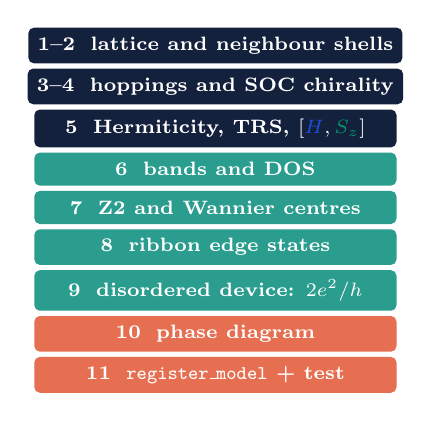
\begin{tikzpicture}[node distance=1.5pt]
\node[st=navy](a){1--2\; lattice and neighbour shells};
\node[st=navy,below=of a](b){3--4\; hoppings and SOC chirality};
\node[st=navy,below=of b](c){5\; Hermiticity, TRS, $[\Hm H,\Sp{S_z}]$};
\node[st=teal,below=of c](d){6\; bands and DOS};
\node[st=teal,below=of d](e){7\; Z2 and Wannier centres};
\node[st=teal,below=of e](f){8\; ribbon edge states};
\node[st=teal,below=of f](g){9\; disordered device: $2e^2/h$};
\node[st=accent,below=of g](h){10\; phase diagram};
\node[st=accent,below=of h](i){11\; \texttt{register\_model} + test};
\end{tikzpicture}
\end{column}
\begin{column}{0.29\textwidth}\centering\fig[width=\linewidth]{lieb_edge.png}\figcap{helical edge states}\end{column}
\begin{column}{0.29\textwidth}\centering\fig[width=\linewidth]{lieb_pd.png}\figcap{Z2 phase diagram vs $\Hp{\lambda},\Hp{\Delta}$}\end{column}
\end{columns}
\vspace{2pt}
{\scriptsize\color{grayt}Weeks \& Franz, PRB 82, 085310 (2010): Lieb-lattice topological insulator, Z2 = 1 at 1/3 and 2/3 filling.}
\end{frame}

% =====================================================================
\section{Status and outlook}

\begin{frame}{Roadmap delivered in v0.8, honest limits, next steps}
\begin{columns}[T]
\begin{column}{0.32\textwidth}
\begin{block}{Delivered (v0.8)}
\scriptsize
\begin{itemize}
\item DMRG / MPS for 100+ site chains
\item GPU back-end (CuPy) for $k$-mesh, Kubo, KPM
\item finite-bias NEGF with self-consistent potential
\item community registry: reference + benchmark per model
\end{itemize}
\end{block}
\end{column}
\begin{column}{0.32\textwidth}
\begin{block}{Current limits}
\scriptsize
\begin{itemize}
\item GPU path verified with a NumPy stand-in for CuPy, not yet timed on a real GPU
\item DMRG without $U(1)$ quantum numbers (sector by penalty or $\mu$)
\item NEGF electrostatics: local Hartree, not full 3D Poisson
\item 40-core scaling measured on few cores; no direct Kwant cross-check
\end{itemize}
\end{block}
\end{column}
\begin{column}{0.32\textwidth}
\begin{block}{Next}
\scriptsize
\begin{itemize}
\item magnon and exchange models from Wannier90
\item symmetric (U(1)/SU(2)) DMRG, iDMRG, TDVP time evolution
\item Poisson solver and inelastic (electron-phonon) NEGF
\item multi-GPU and GPU sparse transport
\end{itemize}
\end{block}
\end{column}
\end{columns}
\end{frame}

{\setbeamercolor{background canvas}{bg=navy}\setbeamercolor{normal text}{fg=white}\usebeamercolor[fg]{normal text}
\begin{frame}[plain,fragile]
\begin{columns}[c]
\begin{column}{0.6\textwidth}
{\Huge\bfseries Get started}\\[14pt]
\begin{lstlisting}[backgroundcolor=\color{white!95!navy},basicstyle=\ttfamily\scriptsize\color{navy}]
git clone https://github.com/Gokaran-Shukla/hopforge
cd hopforge && pip install -e ".[notebooks,test]"
pytest -q
python -m hopforge.benchmarks -j -1
jupyter lab tutorials/
\end{lstlisting}
\vspace{10pt}
{\small\color{white!80}MIT licence \textbullet{} citation in \texttt{CITATION.cff} \textbullet{} contributions of models, benchmarks and quiz questions welcome}
\end{column}
\begin{column}{0.32\textwidth}
\centering

\begin{tikzpicture}\node[fill=white,text=black,inner sep=8pt,rounded corners=4pt]{\color{black}\qrcode[height=3.4cm]{https://github.com/Gokaran-Shukla/hopforge}};\end{tikzpicture}\\[6pt]
{\small github.com/Gokaran-Shukla/hopforge}
\end{column}
\end{columns}
\end{frame}
}

\end{document}
